
%%%%%%%%%%%%%%%%%%%%%%%%%%%%%%%%%%% SETUP
\documentclass{classes/beamer_GeomaticaUA}
%\documentclass[handout]{Classes/beamer_GeomaticaUA}
\usepackage{styles/beamer_GeomaticaUA}
%\usepackage{styles/Amsterdam}
\usepackage{listings}
\renewcommand{\lstlistlistingname}{Codes}
\renewcommand{\lstlistingname}{Code}


%% LISTING ENVIRONMENTS-----------------------
% Java/c#
\lstnewenvironment{Java}{\lstset{
language=Java,                % choose the language of the code
 frame=Ltbr,
 framerule=0.2pt,
 aboveskip=0.5cm,
 framextopmargin=3pt,
 framexbottommargin=3pt,
 framexleftmargin=0.4cm,
 framesep=0.4pt,
 rulesep=0.4pt,
 %backgroundcolor=\color{white},
 rulesepcolor=\color{gray},
 stringstyle=\ttfamily\color{purple},
 showstringspaces = false,
 %basicstyle=\small\ttfamily,
 commentstyle=\color[rgb]{0.133,0.545,0.133},
 keywordstyle=\color[rgb]{0,0,1},%\bfseries 
 %morekeywords={text,serial,with,owner,to, replace, function, for, if, begin, loop, exit,
 %return,returns,cost,row,volatile,into, setof, double, precision,declare,record,reverse,boolean},
 numbers=left,
 numbersep=14pt,
 breaklines=true
}}{}

% SQL
\lstnewenvironment{SQL}{\lstset{
language=SQL,                % choose the language of the code
 frame=Ltbr,
 framerule=0.2pt,
 aboveskip=0.25cm,
 framextopmargin=3pt,
 framexbottommargin=3pt,
 framexleftmargin=0.4cm,
 framesep=0.4pt,
 rulesep=0.4pt,
 backgroundcolor=\color{white},
 rulesepcolor=\color{gray},
 stringstyle=\ttfamily\color{purple},
 showstringspaces = false,
 basicstyle=\tiny\ttfamily,
 commentstyle=\color[rgb]{0.133,0.545,0.133},
 keywordstyle=\color[rgb]{0,0,1},%\bfseries 
 morekeywords={text,serial,with,owner,to, replace, function, for, if, begin, loop, exit,
 return,returns,cost,row,volatile,into, setof, double, precision,declare,record,reverse,boolean},
 numbers=left,
 numbersep=14pt,
 breaklines=true,
 extendedchars=true,
 literate={á}{{\'a}}1 {é}{{\'e}}1 {í}{{\'i}}1 {ó}{{\'o}}1 {ú}{{\'u}}1 {ñ}{{\~n}}1 {¿}{{?`}}1
}}{}


% Defino un entorno CommandLine Linux
\lstnewenvironment{bash}{\lstset{
language=bash,                % choose the language of the code
 frame=Ltbr,
 framerule=0.2pt,
 aboveskip=0.25cm,
 framextopmargin=3pt,
 framexbottommargin=3pt,
 framexleftmargin=0.4cm,
 framesep=0.4pt,
 rulesep=0.4pt,
 backgroundcolor=\color{white},
 rulesepcolor=\color{gray},
 stringstyle=\ttfamily\color{purple},
 showstringspaces = false,
 basicstyle=\tiny\ttfamily,
 commentstyle=\color[rgb]{0.133,0.545,0.133},
 keywordstyle=\color[rgb]{0,0,1},%\bfseries
 morekeywords={cd,mkdir}
 numbers=left,
 numbersep=14pt,
 breaklines=true,
 extendedchars=true,
 literate={á}{{\'a}}1 {é}{{\'e}}1 {í}{{\'i}}1 {ó}{{\'o}}1 {ú}{{\'u}}1 {ñ}{{\~n}}1 {¿}{{?`}}1
}}{}


% PLR
\lstnewenvironment{PLR}{\lstset{
language=R,                % choose the language of the code
 frame=Ltbr,
 framerule=0.2pt,
 aboveskip=0.5cm,
 framextopmargin=3pt,
 framexbottommargin=3pt,
 framexleftmargin=0.4cm,
 framesep=0.4pt,
 rulesep=0.4pt,
 %backgroundcolor=\color{white},
 rulesepcolor=\color{gray},
 stringstyle=\ttfamily\color{purple},
 showstringspaces = false,
 %basicstyle=\small\ttfamily,
 commentstyle=\color[rgb]{0.133,0.545,0.133},
 keywordstyle=\color[rgb]{0,0,1},%\bfseries 
 morekeywords={text,serial,with,owner,to, replace, function, for, if, begin, loop, exit,
 return,returns,cost,row,volatile,into, setof, double, precision,declare,record,reverse},
 numbers=left,
 numbersep=14pt,
 breaklines=true
}}{}

% R
\lstnewenvironment{R}{\lstset{
language=R,                % choose the language of the code
 frame=Ltbr,
 framerule=0.2pt,
 aboveskip=0.5cm,
 framextopmargin=3pt,
 framexbottommargin=3pt,
 framexleftmargin=0.4cm,
 framesep=0.4pt,
 rulesep=0.4pt,
 %backgroundcolor=\color{white},
 rulesepcolor=\color{gray},
 stringstyle=\ttfamily\color{purple},
 showstringspaces = false,
 alsoother={:_\$},
 %basicstyle=\small\ttfamily,
 commentstyle=\color[rgb]{0.133,0.545,0.133},
 keywordstyle=\color[rgb]{0,0,1},%\bfseries 
 %morekeywords={text,serial,with,owner,to, replace, function, for, if, begin, loop, exit,
 %return,returns,cost,row,volatile,into, setof, double, precision,declare,record,reverse},
 numbers=left,
 numbersep=14pt,
 breaklines=true
}}{}

% PHP
\lstnewenvironment{PHP}{\lstset{
language=PHP,                % choose the language of the code
 frame=Ltbr,
 framerule=0.2pt,
 aboveskip=0.5cm,
 framextopmargin=3pt,
 framexbottommargin=3pt,
 framexleftmargin=0.4cm,
 framesep=0.4pt,
 rulesep=0.4pt,
 %backgroundcolor=\color{white},
 rulesepcolor=\color{gray},
 stringstyle=\ttfamily\color{purple},
 showstringspaces = false,
 %basicstyle=\small\ttfamily,
 commentstyle=\color[rgb]{0.133,0.545,0.133},
 keywordstyle=\color[rgb]{0,0,1},%\bfseries 
 numbers=left,
 numbersep=14pt,
 breaklines=true
}}{}

% Diagramas entidad relación
% Ver ejemplo en http://heisenbugs.blogspot.com.es/2010/10/making-great-er-diagrams-without.html
\usepackage{styles/tikz-er2}
\usetikzlibrary{positioning}
\usetikzlibrary{shadows}
\usetikzlibrary{mindmap}
% Diagramas UML
% Ver http://perso.ensta-paristech.fr/~kielbasi/tikzuml/index.php?lang=en
\usepackage{styles/tikz-uml}

%% ER styles
\tikzstyle{every entity} = [top color=white, bottom color=blue!30,
draw=blue!50!black!100, drop shadow]
\tikzstyle{every weak entity} = [drop shadow={shadow xshift=.7ex,
shadow yshift=-.7ex}]
\tikzstyle{every attribute} = [top color=white, bottom color=yellow!20,
draw=yellow, node distance=7em, drop shadow]
\tikzstyle{every relationship} = [top color=white, bottom color=red!20,
draw=red!50!black!100, drop shadow]
\tikzstyle{every isa} = [top color=white, bottom color=green!20,
draw=green!50!black!100, drop shadow]


%% Árboles de directorios
%\usepackage{tikz}
%\usetikzlibrary{trees}

%\tikzstyle{every node}=[draw=black,thick,anchor=west]
%\tikzstyle{selected}=[draw=red,fill=red!30]
%\tikzstyle{optional}=[dashed,fill=gray!50]

%%%%%%%%%%%%%%%%%%%%%%%%%%%%%%%%%%%
%\begin{frame}{Modelo Jerárquico}
%\begin{columns}
%\begin{column}{0.5\textwidth}
%\begin{center}

%\begin{tikzpicture}[%
%  grow via three points={one child at (0.5,-0.7) and
%  two children at (0.5,-0.7) and (0.5,-1.4)},
%  edge from parent path={(\tikzparentnode.south) |- (\tikzchildnode.west)}]
%  \node {País}
%    child { node {Prov A}}		
%    child { node [selected] {Prov C}
%      child { node {Muni C1}}
%      child { node [selected]{Muni C2}
%      	child { node [selected] {Parc 1}}
%      	child { node [selected] {Parc2}}
%      	child { node [selected] {Parc n}}
%      }
%      child [missing] {}	
%      child [missing] {}				
%	  child [missing] {}	
%      child { node [optional] {Muni C$n$}}
%    }
%    child [missing] {}				
%    child [missing] {}	
%    child [missing] {}				
%    child [missing] {}	
%    child [missing] {}							
%    child [missing] {}				
%    child { node [optional] {Prov $n$}};
%\end{tikzpicture}
%\end{center}
%\end{column}
%
%\begin{column}{0.5\textwidth}
%El modelo jerárquico organiza los datos en una estructura ramificada (\textit{tree structure}).\\[3ex]
%
%\textbf{Consulta:}\\
%Cultivos/superficie en el municipio C2\\[3ex]
%
%\textbf{Coste:} \\
%Una búsqueda por Prov, otra por Muni de la Prov C y calculamos las estadísticas para todos. No hay que seguir buscando.
%\end{column}
%\end{columns}
%\end{frame}

%%%%%%%%%%%%%%%%%%%%%%%%%%%%%%%%%%% METADATA
\author{José Torres Prieto}
\title{Introducción Lenguaje de Consultas Estructurado (SQL)}
\titlegraphic{
\includegraphics[height=0.6cm]{logos/logo_ua.png} \hspace{1cm} 
\includegraphics[height=1cm]{logos/iig}} 
\institute[GeomaticaLab]{Instituto Interuniversitario de Geografía\\Laboratorio de Geomática} 
\date{13 de noviembre de 2014}
\subject{Segunda sesión del curso ``Diseño, creación y gestión de Bases de Datos Geográficas con PostGIS''}


%%%%%%%%%%%%%%%%%%%%%%%%%%%%%%%%%%% SLIDES
\begin{document}

\begin{frame}
\titlepage
\end{frame}

\section[Introducción]{Presentación y comentarios}
\subsection{Descripción general del SQL}
\begin{frame}{¿Que vamos a hacer hoy?}
\begin{enumerate}
\item Breve repaso de la sesión anterior y aclaración de dudas
\item ¿Qué es una geodatabase?
\item Caso práctico
\item Teoría y conceptos básicos
\item Diseño de un modelo de datos
\item Implementación en PostGIS
\end{enumerate}
\end{frame}

% --------------------------------------------------- Slide --
\begin{frame}{Introducción a SQL}
\frametitle{SQL}
\begin{block}{¿Qué es SQL?}
El lenguaje de consulta estructurado o SQL (por sus siglas en inglés Structured Query Language) es un lenguaje de acceso a bases de datos relacionales que permite especificar diversos tipos de operaciones en ellas.
Existen tres grupos de operaciones:
\begin{enumerate}
\item DLL - Estructurales - Permiten definir la estructura de la base de datos, tablas, relaciones, índices
\item DML - Consultas - Permiten generar consultas para operar con la base de datos 
\item DCL - Permisos - Permiten definir los permisos sobre los datos
\end{enumerate}

\end{block}
\end{frame}


% --------------------------------------------------- Slide --
\begin{frame}{Operaciones con SQL}
\begin{enumerate}
\item SELECT 
\item UPDATE
\item DELETE
\end{enumerate}
\end{frame}


\section[Consultas SQL]{Ejemplos de consultas complejas con SQL}
\subsection{Modelo relacional y SQL}
%%SQL entre otros lenguajes



%%%%%%%%%%%%%%%%%%%%%%%%%%%%%%%%%%%
\frame{\frametitle{Diagrama Entidad-Relación (físico)}
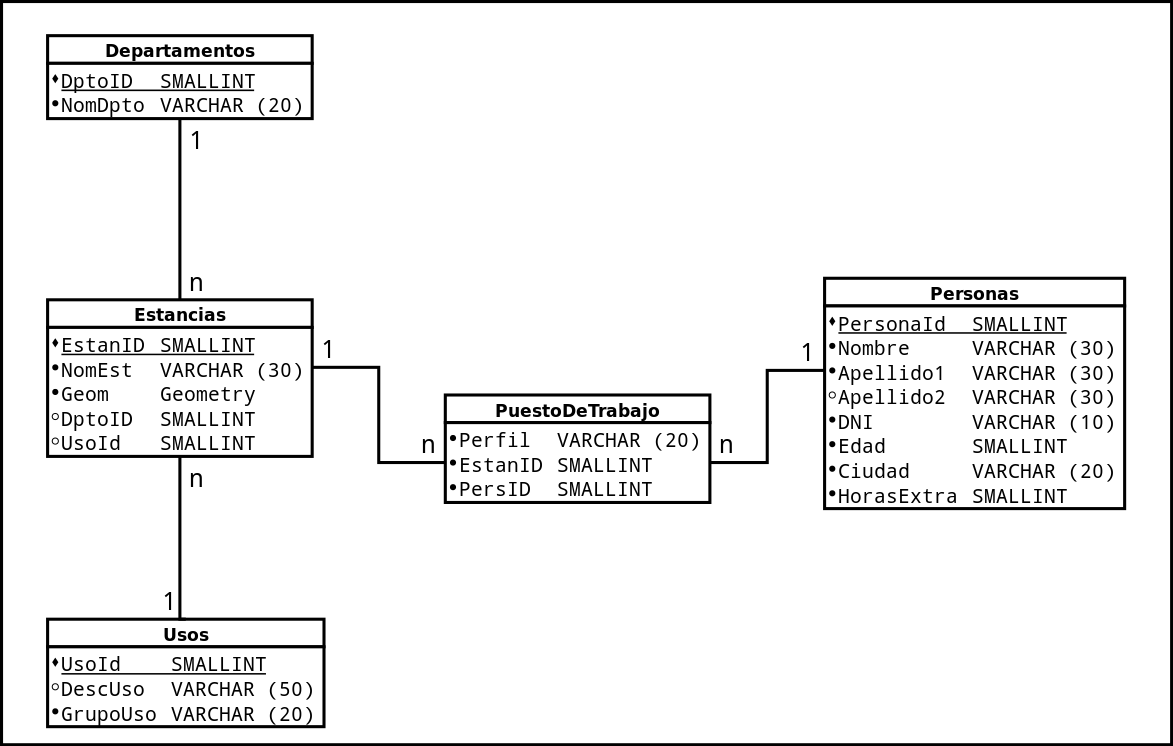
\includegraphics[width=\textwidth]{images/ER.png}
}

%%%%%%%%%%%%%%%%%%%%%%%%%%%%%%%%%%%
\begin{frame}[fragile]
\frametitle{Creación de tablas}

\begin{block}{CREATE TABLE}
Crea una nueva tabla (vacía) en la base de datos actual y admite un buen número de parámetros (tablas temporales, herencia, valores por defecto, OIDs, restricciones, etc). El usuario que haya creado la tabla será el propietario.
\end{block}

\lstset{caption=Crear tabla ``departamentos'',label=sql:crearTablaDepartamentos}
\begin{SQL}
CREATE TABLE departamentos (
DptoID VARCHAR(10) PRIMARY KEY,
NomDpto VARCHAR(50) NOT NULL);
\end{SQL}

\end{frame}


% --------------------------------------------------- Slide --
\begin{frame}[fragile]
\frametitle{Creación de tablas}
%SET DATESTYLE TO 'ISO';
\lstset{caption=Crear tabla ``personas'',label=sql:crearTablaPersonas}
\begin{SQL}
CREATE TABLE Personas (
PersId VARCHAR (20) PRIMARY KEY,
Apellido1 VARCHAR(30) NOT NULL,
Apellido2 VARCHAR(30),
Nombre VARCHAR(30) NOT NULL,
Ciudad VARCHAR (20) NOT NULL,
FechaNac DATE NOT NULL,
HorasExtra SMALLINT DEFAULT 0 NOT NULL);
\end{SQL}
\lstset{caption=Crear tabla ``usos'',label=sql:crearTablaUsos}
\begin{SQL}
CREATE TABLE usos (
CodUso VARCHAR(10) PRIMARY KEY,
DescUso VARCHAR(50),
GrupoUso VARCHAR(20) NOT NULL);
\end{SQL}
\end{frame}


% --------------------------------------------------- Slide --
\begin{frame}[fragile]
\frametitle{Creación de tablas... y tablas con geometrías}

\lstset{caption=Crear tabla ``puestosdetrabajo'',label=sql:crearTablaPuestosdetrabajo}
\begin{SQL}
CREATE TABLE puestodetrabajo (
persid VARCHAR (20) NOT NULL,
estanid VARCHAR (20) NOT NULL,
perfilid VARCHAR (20) NOT NULL,
perfil VARCHAR (50) NOT NULL,
perfilgrupo VARCHAR (20) NOT NULL,
PRIMARY KEY (persid, perfilid));
\end{SQL}



\lstset{caption=Importación de estancias,label=bash:importarEstancias}
\begin{bash}
## Trabajamos en nuestro directorio de usuario
cd
## Descargamos archivo comrpimido con fichero shape de SIGUA
wget https://github.com/labgeo/postgis-intro/raw/2015edition/data/shapefiles/siguapb/siguapb.tar.lz
## Extraemos fichero shape en subdirectorio siguapb
mkdir siguapb; tar --lzip -xvf siguapb.tar.lz -C siguapb
## Importamos a PostgreSQL con la utilidad shp2pgsql
shp2pgsql -s 25830 siguapb/siguapb.shp public.estancias  | psql -h localhost -d ua -U user
\end{bash}


\end{frame}

% --------------------------------------------------- Slide --
\begin{frame}[fragile]
\frametitle{Definir claves externas}

\begin{block}{Mantener la integridad referencial}
Los cambios en una tabla pueden implicar modificaciones en otras tablas relacionadas. PostgreSQL controla esto automáticamente mediante el uso de claves ajenas.
\end{block}

\lstset{caption=Añadir claves ajenas,label=sql:crearForeignKey}
\begin{SQL}
ALTER TABLE estancias 
ADD FOREIGN KEY (coddpto) REFERENCES departamentos(dptoid);

ALTER TABLE estancias 
ADD FOREIGN KEY (coduso) REFERENCES usos(coduso);

ALTER TABLE puestodetrabajo 
ADD FOREIGN KEY (EstanId) REFERENCES estancias(codigo);

ALTER TABLE puestodetrabajo 
ADD FOREIGN KEY (persid) REFERENCES personas(persid);
\end{SQL}


\end{frame}


\section[Ejercicios]{Creatividad con SQL}
\subsection{Ejercicios con JOINS, consultas anidadas, etc}
% --------------------------------------------------- Slide --
\begin{frame}[fragile]
\frametitle{Carga de datos}
\begin{block}{INSERT}
Inserta nuevas filas en una tabla. Se puede insertar una única fila especificada por expresiones de valor, o varias filas, como resultado de una consulta.
\end{block}

\lstset{caption=Insértate en la tabla de Personas,label=sql:insertYourself}
\begin{SQL}
INSERT INTO Personas VALUES('PersId', 'Apellido1', 'Apellido2', 'Nombre', 'Ciudad', 'FechaNac', HorasExtra);
\end{SQL}

Ahora puedes comprobar:
\begin{enumerate}
\item Lo que sucede al introducir un registro con una clave primaria repetida en la misma tabla.
\item Lo que sucede al vulnerar las restricciones especificadas en la creación de las tablas (Ej: Valores nulos o únicos).
\end{enumerate}

\end{frame}


% --------------------------------------------------- Slide --
\begin{frame}[fragile]
\frametitle{Carga de datos masiva}

\begin{block}{COPY}
Utilizaremos este comando para importar y exportar datos entre PostgreSQL y los ficheros del sistema. Este método podrá resultar más práctico y ágil que realizar INSERT.
\end{block}

\lstset{caption=Ejemplo de COPY,label=sql:copy}
\begin{SQL}
-- Para importar datos en ficheros CSV usamos el comando COPY.
-- El comando COPY no es propio del estándar SQL, es específico de PostgreSQL.
COPY departamentos FROM '/home/user/Departamentos.csv' WITH DELIMITER ';' csv header;
-- Ahora importa el resto de ficheros a la base de datos: Usos.csv, Personas.csv y
-- PuestosDeTrabajo.csv
\end{SQL}


\begin{alertblock}{¿Importa el órden?}
Si importas las estancias o los puestos de trabajo antes que las otras tablas te habrá aparecido un error de regla de integridad referencial. No se puede hacer referencia a algo que, por lo que concierne a nuestra base de datos actual, no existe.
\end{alertblock}

\end{frame}


% --------------------------------------------------- Slide --
\begin{frame}[fragile]
\frametitle{Eliminar datos de la DB}

\begin{block}{DELETE}
Este método elimina filas de una tabla que satisfagan la cláusula WHERE o si no hay WHERE, se eliminarán todas las filas de la tabla. El resultado es una tabla válida, pero vacía. Es interesante ver como afecta la existencia de claves ajenas:
\end{block}



\end{frame}


% --------------------------------------------------- Slide --
\begin{frame}[fragile]
\frametitle{Consultas a la BD}

El SQL es un lenguaje estándar de consulta de bases de datos con un gran número de alternativas a la hora de explotar una base de datos. Existen muchos métodos y palabras clave para filtrar, ordenar y combinar los datos. Vamos a practicar un poco:

\lstset{caption=Ejemplos de operadores,label=tab:selects}
\begin{SQL}
SELECT * FROM Personas;
-- SELECT * FROM Personas WHERE Apellido1 = 'tu apellido';
-- SELECT Nombre,Apellido1 FROM Personas WHERE extract(years from age(fechanac)) < 35;
-- SELECT Nombre,Apellido1 FROM Personas WHERE extract(years from age(fechanac)) >= 50 AND extract(years from age(fechanac))<=70;
-- SELECT Nombre,Apellido1 FROM Personas WHERE extract(years from age(fechanac)) BETWEEN 50 AND 70;
-- SELECT NomDpto FROM Departamentos WHERE NomDpto LIKE '%GEO%';
-- SELECT DISCTINCT Perfil FROM PuestoDeTrabajo WHERE Perfil LIKE '%Cate%';
-- SELECT * FROM Personas ORDER BY Apellido1;
-- SELECT Nombre,Apellido1 FROM Personas ORDER BY extract(years from age(fechanac)) asc LIMIT 5 OFFSET 1;

-- Investigad los metodos UNION, INTERSECT y EXCEPT
\end{SQL}

\end{frame}

% --------------------------------------------------- Slide --
\begin{frame}[fragile]
\frametitle{Optimización de consultas}

Dependiendo de la forma de ejecución de una determinada consulta 'select' se consigue reducir de manera significativa el tiempo de ejecución de esta consulta

\input{listings/ejemploOptimizacion}

\end{frame}



\end{document}
